%; whizzy chapter
% -initex iniptex -latex platex -format platex -bibtex jbibtex -fmt fmt
% 以上 whizzytex を使用する場合の設定。


%     Tokyo Debian Meeting resources
%     Copyright (C) 2007 Junichi Uekawa

%     This program is free software; you can redistribute it and/or modify
%     it under the terms of the GNU General Public License as published by
%     the Free Software Foundation; either version 2 of the License, or
%     (at your option) any later version.

%     This program is distributed in the hope that it will be useful,
%     but WITHOUT ANY WARRANTY; without even the implied warranty of
%     MERCHANTABILITY or FITNESS FOR A PARTICULAR PURPOSE.  See the
%     GNU General Public License for more details.

%     You should have received a copy of the GNU General Public License
%     along with this program; if not, write to the Free Software
%     Foundation, Inc., 51 Franklin St, Fifth Floor, Boston, MA  02110-1301 USA

%  preview (shell-command (concat "evince " (replace-regexp-in-string "tex$" "pdf"(buffer-file-name)) "&"))
% 画像ファイルを処理するためにはebbを利用してboundingboxを作成。
%(shell-command "cd image200701; ebb *.png")

%%ここからヘッダ開始。

\documentclass[mingoth,a4paper]{jsarticle}
\usepackage{monthlyreport}

% 日付を定義する、毎月変わります。
\newcommand{\debmtgyear}{2007}
\newcommand{\debmtgdate}{15}
\newcommand{\debmtgmonth}{12}
\newcommand{\debmtgnumber}{35}

\begin{document}

\begin{titlepage}

% 毎月変更する部分, 本文の末尾も修正することをわすれずに


 第\debmtgnumber{}回 東京エリア Debian 勉強会資料

\vspace{2cm}

\begin{minipage}[t]{0.6\hsize}
\vspace{-2cm}
{\fontsize{60}{60}
{\gt
東京エリア \\
デビアン \\
勉強会
}}
\end{minipage}
\begin{minipage}[b]{0.4\hsize}
\hspace{-1cm}
\includegraphics[width=9cm]{image200502/openlogo-nd.eps}
\end{minipage}

\vspace{3cm}
\hfill{}Debian勉強会幹事 上川 純一\\
\hfill{}\debmtgyear{}年\debmtgmonth{}月\debmtgdate{}日

\thispagestyle{empty}
\end{titlepage}

\dancersection{Introduction}{上川 純一}
 
 今月のDebian勉強会へようこそ。
 これからDebianのあやしい世界に入るという方も、すでにどっぷりとつかってい
 るという方も、月に一回Debianについて語りませんか?

 目的として次の二つを考えています。

 \begin{itemize}
 \item メールではよみとれない、もしくはよみとってられないような情報につ
       いて情報共有する場をつくる
 \item Debianを利用する際の情報をまとめて、ある程度の塊として整理するた
       めの場をつくる
 \end{itemize}

 Debianの勉強会ということで究極的には参加者全員がDebian Packageをがりがり
 と作るスーパーハッカーになった姿を妄想しています。

 Debianをこれからどうするという能動的な展開への土台としての空間を提供し、
 情報の共有をしたい、というのが目的です。

\newpage

\begin{minipage}[b]{0.2\hsize}
 \definecolor{titleback}{gray}{0.9}
 \colorbox{titleback}{\rotatebox{90}{\fontsize{80}{80} {\gt デビアン勉強会} }}
\end{minipage}
\begin{minipage}[b]{0.8\hsize}
\hrule
\vspace{2mm}
\hrule
\tableofcontents
\vspace{2mm}
\hrule
\end{minipage}

\dancersection{事前課題}{上川 純一}

今回の事前課題は
「Debian勉強会の目的と照らし合わせて2007年を評価してみた」と「2008年のDebian勉強会のために私はこうします」
というタイトルで200-800文字程度の文章を書いてください。というものでした。
その課題に対して下記の内容を提出いただきました。

\subsection{石原怜美}

\subsubsection{Debian勉強会の目的と照らし合わせて2007年を評価してみた}
 少ししか参加していないのでなんともいえない、です…
 でも、Debian勉強会のことを知り合いに話したら興味を持ってもらえたので
 自分の中ではよし、とします。

\subsubsection{2008年のDebian勉強会のために私はこうします}
 実は、地元に帰ってしまうので、私自身は参加できないのですが、
 友人にがんばってもらいます。
 地元でもちょっと普及の努力をしてみようかな…


\subsection{小室 文}
\subsubsection{Debian勉強会の目的と照らし合わせて2007年を評価してみた}

\begin{description}
 \item[メールでは読み取れない情報について情報共有する場を作る]
これに関してはもっと参加者が分からなかった事などを積極的に聞いたり、ま
 た自分で調べて発表するとか、そういう姿勢が足りなかったと思います。

 \item[Debianの利用方法を整理する場を作る]
 よりよく使う方法と、よりよくする仕組みを作る方法があると思いますが、前
 者にフォーカスしていたので(フォーカスしやすいというのもありますが)、来
 期は2部構成などで、使う方法、作る方法など講義や論議が分かれていたらよい
 かもしれないなーと思いました。
\end{description}

\subsubsection{2008年のDebian勉強会のために私はこうします}

gitを使えるようにします。
Latexでもっと多彩な表現が出来るようにします。
会社の引継ぎをDebian使いにします。
Eximの普及活動もついでにします。
未来のDebian使いを増やします。

\subsection{本庄}

\subsubsection{「Debian勉強会の目的と照らし合わせて2007年を評価してみた」}

「勉強会の目的」を探してみたのですが、どうも見あたらないようでし
た。東京エリアDebian勉強会のウェブページに、背景として「2005年当
初、東京近辺で、類似の勉強会は存在していませんでした。Debian に
ついて語る場所を提供するため、 Debian 勉強会を開催します。」と書
かれており、これが目的に相当するのではないかと思いますが、語る場
として機能していたと思います。

\subsubsection{「2008年のDebian勉強会のために私はこうします」}

風邪で休んでしまったこともあったので、風邪ひかない。

\subsection{山本 浩之}

\subsubsection{「Debian勉強会の目的と照らし合わせて2007年を評価してみた」}

うーむ、2007年の時点では、スーパーハカーにはまだなれていません。

\subsubsection{「2008年のDebian勉強会のために私はこうします」}

こんなわたくしでもお役に立つなら、お手伝いくらいはします。
ただ、現在何が不足していて、どうお手伝いすればいいのかが分からないです。
「雰囲気作りのために、声を出していこー」と、体育会みたいなノリでいいです
かね?
願わくば、講師ができるぐらいのスーパーハカーになれればいいのですが…。

\subsection{前田 耕平}

\subsubsection{「Debian勉強会の目的と照らし合わせて2007年を評価してみた」}
Debian勉強会の本来の目的というと、Debianの開発者を増やす事ですよね。勉強会として今年を振り返ると、年初の勉強会でまずは裾野を広げ、分母を増やして開発者候補を増やそうという目標になった記憶があります。その点については新規参加者が増えたので成果はあったと思います。
自分自身を振り返ると今年は昨年参加し始めたころからますます『お客さん』化しているなと反省。おまけに、未だ自宅鯖もSargeのままだし。

\subsubsection{「2008年のDebian勉強会のために私はこうします」}
初心に返り、当初勉強会に参加しようと思ったきっかけである、HobbitのDebianの公式パッケージ化を目指して、ライセンスあたりが面倒でいつも中途半端になっているDebianパッケージの勉強をちゃんとします。ほいで、完全に放置状態にしてしまった査読を一日10分でもやります。
その前に年内には、この帰っても休みでも仕事な状態を脱しないと。

\subsection{小林儀匡}

\subsubsection{ Debian勉強会の目的と照らし合わせて2007年を評価してみた}
今年の勉強会の目的は、(女子高生などはともかく) 参加者を増やすことだった気がするので、それはクリアできたのではないかと思います。
ただ、参加者を増やしたことが広義の開発者 (公式開発者でなくてもパッケージ管理や翻訳に携わっている人を含む) の増加に繋がっているかといえば、間違いなくNoでしょう。
参加者がガリガリとDebianパッケージのメンテナンスをするような姿を
想像する当初の目的とはずれてきている気がします。

\subsubsection{2. 2008年のDebian勉強会のために私はこうします}
こんなところでしょうか。
\begin{itemize}
 \item  Debian勉強会出身の公式開発者の一人になるべくNew Maintainer (NM) processを進めます
 \item  builddやdakについて勉強して皆さんの前で話をできるようになります。
 \item  もし翻訳関連で何か話すべきことがあれば話をします。
\end{itemize}

\subsection{吉田@板橋}

\subsubsection{Debian勉強会の目的と照らし合わせて2007年を評価してみた}

Debian勉強会の目的とは\url{http://tokyodebian.alioth.debian.org/}から
「Debian について語る場所を提供するため、 Debian 勉強会を開催します。」と
判断しました。

2007年の東京エリアDebian勉強会は、上川さん、岩松さんの毎回の勉強会での
Debianの深いお話、イベントレポート、やまねさんの初心者をDebianに引き込む
プレゼンなどなど、素晴らしいお話を聞ける勉強会でした。元は東京で始まった、
Debian勉強会は関西でも定期的に開催されるようになり、荻窪、代々木、新宿
(OSC)、イギリス エジンバラ、IRC開催等、地域や国、3次元の枠を超え、活動的
ですばらしいです。

\subsubsection{2008年のDebian勉強会のために私はこうします}

私はごくごく一般人のため、Debian勉強会への貢献は難しいとは思いますが、イ
ベントでDebian勉強会関連の冊子の配布に協力させていただいたり、別の勉強会
主催のインストールパーティで何も知らない一般人のPC(のVM上)にDebianをイン
ストールするなどひっそりと協力させていただこうと思います。

\subsection{あけど}


\subsubsection{「Debian勉強会の目的と照らし合わせて2007年を評価してみた」}

今年1年を振り返って、自分に何が出来たのか考えてみました。
\begin{itemize}
 \item  1月一年の計画を立てた。
 \item  2月aptを少し勉強した。
 \item  3月仮想化を少し勉強した。
 \item  4月バージョン管理システムを少し勉強した。 MacにDebianをインストールしてみた。
 \item  5月Etchを少し勉強した。 管理しているDebianマシンをEtchにしてみた。
 \item  6月エジンバラに行ってるメンバーとIRCしようとして挫折
 \item  7月(お休み)
 \item  8月cdn を少し勉強した。BSPに参加、少し査読。・・・って残りがまだあった! orz
 \item  9月(お休み)
 \item  10月OSCで盛り上がった。
 \item  11月(お休み)
\end{itemize}
後半は何かと忙しくて時間が取れなかったこともあり、殆ど何も出来てません。
点数でいえば20点くらい?
やりたかった事は何もできてませんので、
来年はもう少し計画的にやって何か出来たという風にしたいです。

\subsubsection{「2008年のDebian勉強会のために私はこうします」}
今年の反省を踏まえ、自分に出来そうなことをやっていきたいです。
1つは、マニュアルのレシピ化というのを考えています。
いわゆる事例集のようなものですが、
各コマンドの実行例とコマンドオプションのポイントといったものを
まとめてみたいと思います。
来年の後半には何らかの発表が出来るようにしたいと思います。

\subsection{山本 琢}

今年勉強会で実現できたこと:\\
 オープンソースのカルチャーに触れて、オープンソース開発に興味を持てた。

来年勉強会で実現したいこと:\\
 実際にオープンソース開発プロジェクトに貢献(パッチを投げられる)し、その
過程や成果についての報告や、アドバイスが受けれるようにしたい。

\subsection{キタハラ}

\subsubsection{「Debian勉強会の目的と照らし合わせて2007年を評価してみた」}

  お題を見て、改めて勉強会のWebページを見たの
ですが、「背景」はありますが「目的」はないですね。
(見落としている?) 「背景」にある「Debian につい
て語る場所を提供するため」というのが目的だとすると、
有識者の方に大いに語って戴いて、(私の理解の範囲外
なものもありましたが)多くの有用な知識を得ることが
出来て、私にとっては(勉強会の後の懇親会も含めて)
大変有意義であったと思います。

  真の目的(?)にはまったく貢献していませんが、
無能が故ということでお許しください。

\subsection{上川 純一}

Debian勉強会の目的と照らし合わせて2007年を評価してみたところ、
自由の戦士(Debian Developer)を量産することが目的だったのに、第3次自由の
戦士量産計画は成果を出せずに終了しました。ふがいない。

「2008年のDebian勉強会のために私はこうします」という観点からいうと、
もしかして、NMキュー通過のためのブートキャンプなどをすればよいんじゃない
か?

%%% trivia quiz
\dancersection{Debian Trivia Quiz}{上川 純一}

ところで、みなさん Debian 関連の話題においついていますか?Debian関連の話
題はメーリングリストをよんでいると追跡できます。ただよんでいるだけではは
りあいがないので、理解度のテストをします。特に一人だけでは意味がわからな
いところもあるかも知れません。みんなで一緒に読んでみましょう。

今回の出題範囲は\url{debian-devel-announce@lists.debian.org} に投稿された
内容からです。
\begin{multicols}{2}
 
 \subsection{問題}

 \santaku
 {Debian Developer になる前の人たちのための制度で最近 Open Beta を開始したのは何か}
 {Debian Maintainers}
 {Ubuntu}
 {Debian Account Manager}
 {A}

 \santaku
 {Debian Auditor は誰か}
 {Kalle Kivimaa}
 {Anthony Towns}
 {Sam Hocevar}
 {A}

 \santaku
 {Anibal Monsalve Salazar が参加したのはどのチームか}
 {Debian System Administrator}
 {Debian Cabal}
 {Debian Maintainer Keyring Team}
 {C}

 \santaku
 {debian/control に追加された Vcs-* フィールドでないのはどれか}
 {Vcs-git}
 {Vcs-rcs}
 {Vcs-Mtn}
 {B}

 \santaku
 {debian/control でパッケージのアップストリームプロジェクトのURLを記述す
 るためのフィールドは}
 {Homepage:}
 {URL:}
 {Upstream:}
 {A}

 \santaku
 {dpkg-buildpackage で並列ビルドをするためのコマンドラインオプションは}
 {-rfakeroot}
 {-j}
 {--nori1}
 {B}

 \santaku
 {2009年開催予定のDebconf9 の場所が発表された、その場所は}
 {Osaka}
 {Tokyo}
 {Extremadura}
 {C}

 \santaku
 {Policy 3.7.3.0 で追加されなかった変更は}
 {バージョン番号にチルドが利用できるようになった}
 {自由でないものはパッケージではない}
 {Debconf を利用する場合は国際化対応必須}
 {B}

 \santaku
 {gnuab にかわるリリースされていないDebian移植版のホスティングの場所はど
 こか}
 {http://www.debian-doorstop.org/}
 {http://www.debian-ports.org/}
 {http://www.ubuntu.org/}
 {B}

\end{multicols}

\dancersection{最近のDebian関連のミーティング報告}{上川 純一}
\subsection{東京エリアDebian勉強会34回目報告}

% (query-replace-regexp "<.*?>" "")

	  11月の第34回東京エリアDebian勉強会を実施しました。
	  	  今回の参加者は
	  山本浩之さん、小林さん、前田さん、satokenさん、キムラオサムさん、Mattia、Ester Celli、荒木淳さん、
	  山本琢さん、やまねさん、でんさん、福田朝さん、本庄さん、キタハラさん、イアンルイスさん、千葉さん、岩松さん、野首さん、上川の19人でした。
        
	
	  
	    まず、クイズを今回も実施しました。
	    今回もDWNが出ていないので、debian-devel-announce の内容から出題しました。
	    最後までのこった3人に特製のDebian関連の豪華景品が渡されました。
	  
	  
	    最近のイベントについては、Biella Coleman の宴会についての報告を行いました。
	  
	  
	    事前課題の紹介をしました。
	    サーバ関連については思うところがたくさんあるようで、文字数の制限にありったけの思いをみなさんつっこんでいました。
	    よい点が多数あるけど、不満もあるようです。
	    自動インストールの仕組み preseed についてはあまり試している人がいないようで、ぜひためしてみたいものです。
	  
	  
	    岩松さんが live-helper についての紹介をしました。
	    細かい設定方法、ソースをよまないとおいついていけないような活発な開発状況などがあるそうですが、
	    現状のlive-helper の使い方についての情報が整理されていました。
	    試してみる人が増えることで日本語の情報が増えるとよいですね。
	  
	  
	    野首さんが bluetooth のデバイスの使い方について紹介しました。
	    市販のデバイスはPINが固定のものが結構あり、0000になっているものなのが多いようです。
	    hcitool とかを駆使して設定するようです。
	    google docs をつかってプレゼンテーションをしていました。
	    また、岩松さんが野首さんのbluetoothマウスを乗っ取られる実演までしていました。
	  
	  
	    山根さんが TOMOYO Linux Kernel Patch パッケージを作成した際の体験談を語りました。
	    dh-kpatches で実は結構簡単にできるということがわかりました。
	    ただし、カーネルパッチは、元のカーネルが頻繁に大幅に変更されるもので、
	    どのパッチがどのバージョンにあたってそれがどう動作するのかはたして確認できるのか、という点で議論が紛糾しました。
	    Debian としてカーネルパッチが提供されているのだから、パッチが適用するレベルまでは確認するべきか、
	    はたまたビルドして動作するところまで確認するべきか。
	    Debian Project としてはユーザが色々と試してバグ報告をすることに依存しているので、ぜひユーザのパワーを見せつけていただきたい所です。
	  
	  
	    上川がOSC Tokyo/Fall でのイベントの報告をしました。
	    サーバ機器 ML350G5 と ML110G4 を試してみましたが、結局特殊な技は全然試せていません、ということで終わりました。
	    会場は Eyetoy がどこに売っているのか、ということで盛り上がりました。
	  
	  
	    今回は宴会は時の居酒屋 刻 荻窪店にて開催しました。終電までみ
	      んなで宴会しました。みんな無事にかえれたかな?


\dancersection{東京エリアDebian勉強会の設計}{上川 純一}
\label{sec:debmtg2007design}

\index{debianjp@Debian JP} 
\index{とうきょうえりあ@東京エリアDebian勉強会}

Debian勉強会はDebianの日本における発展を支援するために実施しているイベン
トです。Debian勉強会を運営している上での仮説を説明します。勉強会はこの仮
説に基づいて運営しています。まず前提条件を整理したのち、現状の状況を分析
して、Debian勉強会からどういう成果が期待できるのかを整理します。

\subsection{Debian JP とは}

Debian Project メンバーの日本在住の有志およびDebian Projectの Debian
Developer になる候補者で構成されているのがDebian 開発者の会(Debian JP)
です。Debian JP の会員はどういう人が存在しているのか、という点を議論した
ところ、下記の分類があぶり出されました。

\begin{itemize}
 \item Debian JPの会員は開発・翻訳・インフラを担当している人により構成さ
	れています。過去の経緯により、既存の会則・方針では、Debian JP は
	「開発者の会」という位置づけのため、「ユーザ」については Debian
	JP 「会員\footnote{Debian 開発者の会の「会員」は会則に定義されて
       おり、例えば投票する義務のある人のことです}」ではありません。
 \item 開発者とは Debian JP で開発を行っている人、パッケージ・スポンサー
	されている人、New Maintainer、 Debian Developer などをいいます。
 \item インフラは、Debian JP の運営に必要なインフラで ftp, www, svn, ML,
       LDAP などをいいます。
\end{itemize}

\begin{figure}[h]
\begin{center}
  {\large
 \begin{tabular}[t]{|c|c|c|}
 \hline
 \rotatebox{90}{ユーザ }& \rotatebox{90}{開発者 }&\rotatebox{90}{翻訳者 } \\
 \hline 
 \multicolumn{3}{|c|}{インフラ}\\
 \hline
 \end{tabular}
 }
\end{center}
 \caption{Debian JP のメンバー要素分類}
\label{fig:debianjpmemberitem}
\end{figure}

Debian JP の目的としては、いろいろありますが、Debianの日本の開発者
(Debian Developer)のコミュニティーとなることを目指しています。また日本
におけるDebianの代表・とりまとめとしての役割をになっており、Debianが日本
で利用しやすくなることの促進を行っており、翻訳作業のとりまとめや、外国か
らDebian Developerが来訪したときの宴会調整の連絡先として機能していたりし
ます。また、Debianの商標を管理していたりします。



Debian JP が成功すると、Debianの日本語対応がよくなり、日本にいるDebian
Developerがふえ、日本にいるDebianユーザがふえ、日本でDebianを使うことがや
りやすくなるはずです。

Debian JP の目的から考えると、開発者のコミュニティーとしての機能、および
ユーザとの情報交換の機能の部分を保管するのが東京エリアDebian勉強会でしょ
う。また、今後のDebian Developer候補の発掘・育成(・そそのかし)のために
活動すればよいでしょう。




\subsection{Debian JP の各種会議体の位置付け}

Debian Projectには各種組織、および会議体が存在します。東京エリア Debian
勉強会を中心に、それらの関係を整理してみます。

「東京エリア Debian 勉強会」はDebian Projectの日本における組織である
Debian JP が主体となり、「東京エリア Debian 勉強会幹事」に委任して開催し
ているイベントです。目的としているのは、Debianのパワーユーザと既存の開発
者層に着目し、Debian Developerの育成、および翻訳活動に参加できる人たちへ
の情報提供、および必要な情報の交換です。

\includegraphics[width=1\hsize]{image200712/debianmeetinganddebianjp.eps}

各種定期的に開催している会議体を整理してみます。

\begin{tabular}[t]{|l|l|p{14em}|p{12em}|}
\hline
会 & 開催頻度 & 目的 & 参加者層 \\
\hline
総会・選挙 & 年一回 & Debian JP 内部の運営方針の策定 & Debian JP 会員 \\
OSC & 年数回 & 新規ユーザ発掘・公報 & OSCの一般参加者 \\
東京エリアDebian勉強会 & 月一回 & Debian 開発者の新規発掘と支援 & Debian の開発者をめざす東京近辺在住の
 メンバー \\
関西Debian勉強会 & 月一回 & Debian ユーザ・開発者の新規発掘と支援 & Debian を使う大阪近辺
	     在住のメンバー\\
IRC定例会議 & 月に二回程度 & Debian JPの運営に関する情報共有と意思決定 & Debian JP
 会員 \\
\hline
\end{tabular}

会議の情報が伝達される経路について整理してみます。Debian JPで
利用している主な情報交換の方法を整理してみました。各種の会議が開催され、
成果が報告されます。参加したメンバーが情報を得られるのはもちろんですが、
参加していないメンバーもなんらかの情報が取得できます。事前資料は公開され
るため、ウェブで取得できます。また、その他の情報取得の手段があります。

\includegraphics[width=1\hsize]{image200712/debianjpandmedia.eps}


\subsection{東京エリアDebian勉強会においての事前資料の意義}

「事前資料」は記録性、参照性を重視しています。2007年12月の「事前資料」は
当日の勉強会でも利用しますが、今年の勉強会の幹事・講師をしてくれる人の説
明資料としても随時利用します。「これを読めば何をすればよいかがわかる」と
いう形にしたいと思っています。プレゼンテーションに利用する資料は若干毛色
が違い、議論をするためのフレームワークを提供するものだと考えています。

「事前資料」については、勉強会で紙の媒体の資料として利用するのと、コミッ
クマーケットを契機として「アンドキュメンティッド Debian」として再度編集
し、半年に一度まとめて製本します。そのことで、知識の精査、定着と展開がは
かれることを目的としています。

\subsection{事前課題の役割}

東京エリア Debian 勉強会では、ただのセミナー参加でおわることは期待してい
ません。理想的な最終目標としては、Debian Developer としてばりばりと貢献で
きるような意識の高い参加者を求めています。そこまでの理想を追い求めるのは
現実的ではないにしても、何も準備せずに参加するより、何らかの心構えをして
参加してもらった方がよいだろうということで、毎回事前課題を設定しています。
いろいろなアイデアが出てきておもしろいです。

参加する際には事前課題は必須ということにしています。今年の参加者の事前課
題の提出率を見ると半分以上が提出していることが分かります。

\begin{table}[h]
 \caption{2007年の事前課題}
 \begin{center} 
  \begin{tabular}{|l|c|c|p{20em}|}
 \hline
 & 参加人数 & 事前課題提出人数 & 内容\\
 \hline
 2007年1月 & 15 & 6 & 今後、勉強会につかう施設を提案してください、2007年の勉強会の各月のアジェンダを提案してください\\
 2007年2月 & 13 & 8 & aptに足りなさそうな機能, パッケージングをしてみて感じたこと、または何故パッケージングをしないか\\
 2007年3月 & 80 & 6 & 仮想化を実際にこういう利用方法で活用しています\\
 2007年4月 & 19 & 14 & 私はバージョン管理システムをこのようにつかっています \\ 
 2007年5月 & 23 & 14 & 「エッチになって困った事」 \\
 2007年6月 & 4 & & \\
 2007年7月 & 18 & 12 & 今後Debconfを日本で開催するためにDebianの認知度を上げる方法、企業がDebconfのスポンサーになるためには \\
 2007年8月 & 25 & 18 & ここ最近 Debian を使っていて ハマったこと/ちょっと
	       感激したこと、apt の sources.list はこう書く\\
 2007年9月 & 14 & 7 & 「あなたがDebianで使っている MTA のこだわりの設定」もしくは「Debian 
 で利用しているこんな便利な/楽しいメッセージツールあるいは日頃使っていて
 気にかかるメッセージ関連ソフトのこの部分」\\
 2007年10月 & 30 & & \\
 2007年11月 & 19 & 10 & 「Debian の Live CD ってこんなふうに使ってます」もしく
	   は「ノートPCやデスクトップPCではなく、サーバ機器での Debian
	   に期待するものって何?」\\
 2007年12月 & 11 & 11 & 「Debian勉強会の目的と照らし合わせて2007年を評価してみた」と「2008年のDebian勉強会のために私はこうします」 \\
 \hline
  \end{tabular}
 \end{center}
\end{table}

\subsection{12月の勉強会の役割}

毎年の忘年会をかねて東京エリアDebian勉強会の12月開催は、一年間を反省する
会を開催しています。12月号の事前資料は、運営に関連する情報を共有するため
に準備しています。ターゲットは幹事・講師で、その説明文を見ることで講師や
幹事が何をどういう理由で実施する必要があるのかを理解できることを目的とし
ています。内容については定期的に修正が必要なものなので、毎年12月の資料と
して新規に作成しています。勉強会の目的は通常と違い、勉強会の実績の確認と、
今後の方向性の策定だけをするという会にしています。

\dancersection{東京エリア Debian 勉強会のワークフロー}{上川 純一}
\label{sec:debmtg2007workflow}

\index{debianjp@Debian JP} 
\index{とうきょうえりあ@東京エリアDebian勉強会}

東京エリア Debian 勉強会は事前に会場も日時も決定してしまっています、その
ため資料の準備・告知・予約などができる期限が決まっています。Debian 勉強会
では月に二回行われる Debian JP IRC 定例会議と、幹事用のメーリングリストを
利用して進捗の管理をしています。開催直前の最後の一週間はタイトになります。
ワークフローの内容をみてみましょう。git レポジトリの
\url{planner/200704-tokyo.ods} にファイルが置いてあります。

毎月の作業は次のようなものがあります。
\begin{description}
\item[会場確保]  勉強会の会場を予約します。2ヶ月前程度に予約しないと大抵
	   の会場はうまってしまいます。日程については年間スケジュールを
	   事前に確定しておき、それから若干の調整をかける形にするのがよ
	   いでしょう。
\item[企画立案] 企画を立案します。前回の勉強会の宴会、もしくは年初の企画
	   会議などで決定します。
\item[講師確保] 前回の勉強会であたりをつけて、講師候補のメールで調整する
	   ようにします。
\item[資料作成依頼] 資料の作成を講師に依頼します。資料の作成の方法につい
	   ての資料も必要でしょう。
\item[資料作成] 講師が資料を作成します。git レポジトリを活用して共同作業
	   をするのがよいでしょう。
\item[資料編集] 資料を集めて資料を編集します。元の資料が \LaTeX{}でない
	   場合には\LaTeX{}形式にする作業などがあります。ページ数にあて
	   はまるようにする、用語を統一する、誤字脱字を修正する、などの
	   対応を行います。
\item[印刷向け編集(4の倍数)] 冊子として印刷に出すときに紙は4ページの
	   倍数である必要があります。そのために技を駆使します。内容をけ
	   ずったり、画像の位置を微調整したり、フォントを小さくしたり、
	   文章が一行におさまるように書き直したり、などの技があるようで
	   す。
\item[kinkos印刷依頼] kinkos に印刷を依頼します。ウェブ経由でお願いする
	   ことができます。\url{http://www.kinkos.co.jp/}からアクセスし
	   て、「オンラインプリント」のメニューを選択します。半日程度
	   (12時間)は余裕をみてあげるのがよいでしょう。
\item[kinkos印刷受け取り] 印刷したものを受け取ります。面倒ですが、確認の
	   意味も含めて、直接うけとって支払
	   うのがよいでしょう。
\item[事前課題設定] 参加者に事前に考えてきてほしい内容を設定します。勉強
	   会の次回の企画テーマにあうようなものがよいです。またハードル
	   が高すぎると参加者がこまっちゃうので気を付けましょう。
\item[事前課題提示] 事前課題をウェブページに提示します。
\item[資料反映] 資料を反映します。
\item[DWN Quiz作成] クイズを作成します。わからないとどうしようもないので、
	   わかりやすいものをこころがけましょう。
\item[DWN Quiz景品準備] 何か景品を準備しましょう。
\item[案内文文書案作成] 案内文の素案を作成します。見た人が参加したくなる
	   ように、また参加して意味のある人が参加できるように、何を期待
	   したらよいかを明確にします。これは幹事MLでレビューにまわしま
	   す。
\item[案内文確定] レビューした後、案内文を確定します。各種メディアに展開
	   します。
\item[aliothウェブ掲載] alioth のウェブページに掲載します。
\item[debian.or.jp掲載] debian.or.jp のウェブページに掲載します。
	   掲載の方法については
	   \url{http://www.debian.or.jp/community/translate/webmasters.html}
	   を参照。
	   \texttt{www/trunk/src/community/events/index.tt2} のイベント
	   の一覧に追加し、 \texttt{www/trunk/blosxom/data/} に blog エントリーを追加
	   します。
\item[mixi掲載]  mixi の debian コミュニティーに掲載します。\url{http://mixi.jp/view_community.pl?id=95}
\item[debian-devel投稿]
	   Debian JPのメーリングリスト \url{debian-devel@debian.or.jp},
	   \url{debian-users@debian.or.jp} に投稿します。
	   二週間前ごろをメドにします。
\item[debian-devel再度投稿]
	   数日前に再度投稿します。
\item[予約システムの作成]
	   宴会くん \url{http://utage.org/enkai/}などを利用し、
	   予約用のエントリーを作成します。これは3週間前くらいにはつくっ
	   ておきます。
	   
\item[参加者把握]
	   数日前に参加者を把握しておきます。
\item[出席簿印刷]
	   当日のために出席簿を印刷します。
\item[宴会予約]
	   宴会の場所を予約します。場所によりますが前日までに予約したほ
	   うがよいです。店に電話で直接連絡します。
\item[宴会費回収] 宴会を開催、代金を回収します。5000円、4000円などのきり
	   のよい金額が会費として徴収できるように調整します。東京Debian
	   勉強会では講師をしてくれた人に関しては徴収しないようにしてい
	   ます。
\item[会場設置] 会場を設置します。事前に幹事がはやめに入ることが必要です。
	   一人ではできないので、手伝ってくれる人がきてくれないと困るな。
\item[出席確認] 会費を徴収し、資料を配布します。受付担当者としては、参加
	   者の方の名前を覚えるチャンスです。
\item[結果報告書整理] 
	   実際に今回どういう会だったのかということを整理し、報告にまと
	   めます。
	   \url{http://tokyodebian.alioth.debian.org/}
	   ウェブページから反応リンク集という形でまとめ、
	   Debian JP IRC会議にて内容を報告します。
\end{description}

年間一度している作業内容は次のようなものがあります。
\begin{description}
\item[年間スケジュール設定] 一年間のスケジュールを決定します。内容につい
	   てはあまり重要ではありませんが、会場の予約のためには日程が決
	   まっていることが重要です。
\item[前年度の内容確認] 出席者の傾向、開催内容の傾向と参加者数の増減、
	   Debian JPの傾向などを分析し、どういう状況で、何が行われたのか、
	   を確認します。
\item[tokyodebian-XXX ML作成] 事前課題を投稿してもらっているメーリングリ
	   ストを再設定します。
\end{description}


\dancersection{東京エリア Debian 勉強会資料の準備の方法}{上川 純一}
\label{sec:debmtg2007howtoprepare}
\index{debianjp@Debian JP} 
\index{とうきょうえりあ@東京エリアDebian勉強会}

\subsection{文章ルール}

文章は敬体に統一しましょう。

固有名詞は基本としては敬称略、フルネーム、で記述しましょう。日本名称の場
合、苗字と名前の間には半角の空白を一文字入れます。

\subsection{レポジトリの取得}

まず最初にgitのレポジトリを取得します\footnote{git の使いかた詳細につい
ては、2007年4月の勉強会資料を参照してください。 apt-get install git-core
でインストールできます。} 。読み込み専用であれば、
git プロトコル、もしくは、http プロトコルでよいでしょう。書き込み権限を
持っているのであれば、ssh プロトコルを利用すれば直接 git push でアクセス
することができます。


\begin{commandline}
 git clone git://git.debian.org/git/tokyodebian/monthly-report.git
 git clone http://git.debian.org/git/tokyodebian/monthly-report.git
 git clone ssh://git.debian.org/git/tokyodebian/monthly-report.git
\end{commandline}

この結果、カレントディレクトリに monthly-report というディレクトリができ
ます。
monthly-report/.git 以下がレポジトリです。
git の使いかたについては 4 月の資料を参照してください。

\begin{commandline}
$ ls -la monthly-report/ | head
合計 2500
drwxr-xr-x 28 dancer dancer   1960 2007-04-22 09:46 .
drwxrwxrwt 17 root   root      560 2007-04-22 09:46 ..
-rw-r--r--  1 dancer dancer    168 2007-04-22 09:46 .cvsignore
drwxr-xr-x  8 dancer dancer    240 2007-04-22 09:46 .git
-rw-r--r--  1 dancer dancer     61 2007-04-22 09:46 .gitignore
-rw-r--r--  1 dancer dancer     71 2007-04-22 09:46 .whizzytexrc
-rw-r--r--  1 dancer dancer    145 2007-04-22 09:46 .yatexrc
-rw-r--r--  1 dancer dancer  17989 2007-04-22 09:46 COPYING
-rw-r--r--  1 dancer dancer  25069 2007-04-22 09:46 ChangeLog
\end{commandline}
%$

\subsection{コミットの方法}

まず、PDFファイルが生成できることを確認します。Makefile があるので、make 
コマンドを入力するとビルドしてくれるはずです。
文字コードが正しいか、正常にビルドできるか、などのチェックが組み込まれて
いるので、チェックに活用しましょう。

\begin{commandline}
 make
\end{commandline}

その後、git diffでコミットされる内容を確認します。意図している内容が表示
され、問題ないようであれば、git commit コマンドでコミットします。手元のレ
ポジトリに反映されます。

\begin{commandline}
 git diff
 git commit -a -m 'revised XXX'
\end{commandline}

問題がないようであれば、git pull / git push でマージします。git-pull し
た後にコンフリクトが発生したら、修正し、git commit でコミットしてから
git push します。

\begin{commandline}
 git pull 
 git push 
\end{commandline}

新規のファイルを追加する場合、ファイルを削除する場合には、 git add /
git rm コマンドを利用します。

\subsection{ファイルの編集}

\index{latex@\LaTeX}
ドキュメントは p\LaTeX{}で作成しています。ファイル名として下記になってい
ます。(YYYY)(MM)は、年と月で、例えば2007年12月であれば 200712 です。

\begin{description}
 \item[debianmeetingresume(YYYY)(MM).tex]
	    事前配布資料
 \item[debianmeetingresume(YYYY)(MM)-presentation.tex]
	    プレゼンテーション用 (prosperを利用)
 \item[image(YYYY)(MM)/]
	    画像ファイルなどの置き場
\end{description}


作業する前にビルドに必要なパッケージをインストールします。

\begin{commandline}
# tex から PDF の生成関連
apt-get install ptex-bin dvipdfmx latex-beamer \
 okumura-clsfiles gs-esp xpdf xpdf-japanese
\end{commandline}

編集に便利なツールもついでにインストールしてみてもよいでしょう。

\begin{commandline}
 apt-get install whizzytex advi emacs21 yatex gs-cjk-resource gv
\end{commandline}

tex4ht を利用して HTML 出力をさせる場合は下記もインストールしたらよいで
しょう。ただし、2007年8月現在、dvi2ps-fontdata-a2n の影響で dvi 出力ができなくな
る副作用があります。

\begin{commandline}

# tex4ht での HTML 生成関連
apt-get install dvi2ps-fontdata-a2n dvi2dvi dvipng tex4ht
\end{commandline}

文字コードは iso-2022-jp で統一しています\footnote{Windows 版と Linux 版
の ptex で共通して扱える文字コードにしたという経緯があります。ただし現状
Windows で全部できる状況ではありません。}。たとえば、emacs + yatex を使用
している場合で iso-2022-jp をデフォルトにするには、下記のような設定を
\texttt{.emacs} にかけばよいでしょう。

\begin{commandline}
(add-hook 'yatex-mode-hook
	  '(lambda () 
	     (progn 
	       (if (string-match "^/home/user/tokyodebian/" default-directory)
		   (progn (set-buffer-file-coding-system 'iso-2022-jp)
			  (set-buffer-modified-p nil))))))
\end{commandline}


emacs での編集で、outline-mode を利用すると、アウトラインをベースに編集す
ることができ、便利です。tex ファイルの最後に以下のようなエントリーを追加
しています。
M-x outline-minor-mode で有効にできます。

\begin{commandline}
;;; Local Variables: ***
;;; outline-regexp: "\\([ <タブ記号>]*\\\\\\(documentstyle\\|documentclass\\|<改行しない>
dancersection\\)\\*?[ <タブ記号>]*[[{]\\|[%<^L>]+\\)" ***
;;; End: ***
\end{commandline}

\begin{itemize}
 \item 
 \verb!<タブ記号>!: タブを入力、
 \item  \verb!<^L>!: ctrl-L を入力、
 \item  \verb!<改行しない>!: ここの改行はみやすいように改行をいれているだけで、実際には改行は入力しない。
\end{itemize}

また、自動で適切な設定で outline-minor-mode に入るように .emacs に設定してもよいでしょう。

\begin{commandline}
(add-hook 
 'yatex-mode-hook
 '(lambda ()
    (make-variable-buffer-local 'outline-regexp)
    (setq outline-regexp 
	  "\\([ \t]*\\\\\\(documentstyle\\|documentclass\\|chapter\\|dancersection\\|
section\\|subsection\\|subsubsection\\|paragraph\\)\\*?[ \t]*[[{]\\|[%\f]+\\)")
    (setq 
     outline-level 
     (function
      (lambda ()
	(save-excursion
		   (looking-at outline-regexp)
		   (cond 
		    ((equal (char-after (match-beginning 0)) 37) (- (match-end 0) (match-beginning 0)))
		    (t (let ((bs (buffer-substring (match-beginning 2) (match-end 2))))
			 (cond ((equal (substring bs 0 2) "do") 15)
			       ((equal (substring bs 0 1) "c") 0)
			       ((equal (substring bs 0 1) "p") 4)
			       ((equal (substring bs 0 2) "da") 1) ; dancersection
			       ((equal (substring bs 0 2) "se") 1) ;section
			       ((equal (substring bs 0 5) "subse") 2) ;subsection
			       ((equal (substring bs 0 8) "subsubse") 3) ;subsubsection
			       (t (length bs))))))))))
    (outline-minor-mode t)))
\end{commandline}

\subsubsection{ドキュメントのスタイル}

スタイルファイルは monthlyreport.sty パッケージを利用します。過去の資料を参考にしてください。

\begin{commandline}
\usepackage{monthlyreport} 
\end{commandline}

各担当部分は section として扱います。特別なコマンド dancersection で指定
します。形式は \texttt{dancersecion\{タイトル\}\{作者名\}}です。
その中で subsection や subsubsection を利用して文書を構成してくださ
い。

\begin{commandline}
 \dancersection{Debian 勉強会資料の準備の方法}{上川 純一}
 \label{sec:debmtg2007howtoprepare}
\end{commandline}

\subsubsection{目次の処理}

目次のエントリは下記の形式で作成します。
\begin{commandline}
index { alphabet もしくは、 ひらがなの読み @ 項目名称 } 
\end{commandline}

\subsubsection{画像ファイルの処理}

画面写真の画像を追加するときは、できるだけサイズの小さい png などを利用
してください。グラフなどの線画であれば、epsでかまいません。png であれば、 
ebb コマンドを利用してbounding box を作成してください。

\begin{commandline}
 ebb XXX.png
\end{commandline}

ps であれば、 eps2epsでバウンディングボックスを追加してあげるとうまくい
きます。sodipodi の出力する ps を eps2epsで処理すれば sodipodi で画像を
作成することができます。

\subsection{pLaTeX+latex-beamerで文書作成}

latex-beamer で生成したファイルは現状 whizzytex+advi でプリビューできませ
んが、gv, もしくは xpdf を利用してプリビューすることは可能です。gv を利用
する場合は最初の行に ps モードを指定してください。advi のように自動で編集
しているページにとんでくれはしませんが、自動リビルド、および自動更新はか
かります。

\begin{commandline}
 %; whizzy document -ps gv
\end{commandline}

xpdf を利用する場合は下記のように設定します。

\begin{commandline}
 %; whizzy section -pdf xpdf -latex ./whizzypdfptex.sh
\end{commandline}

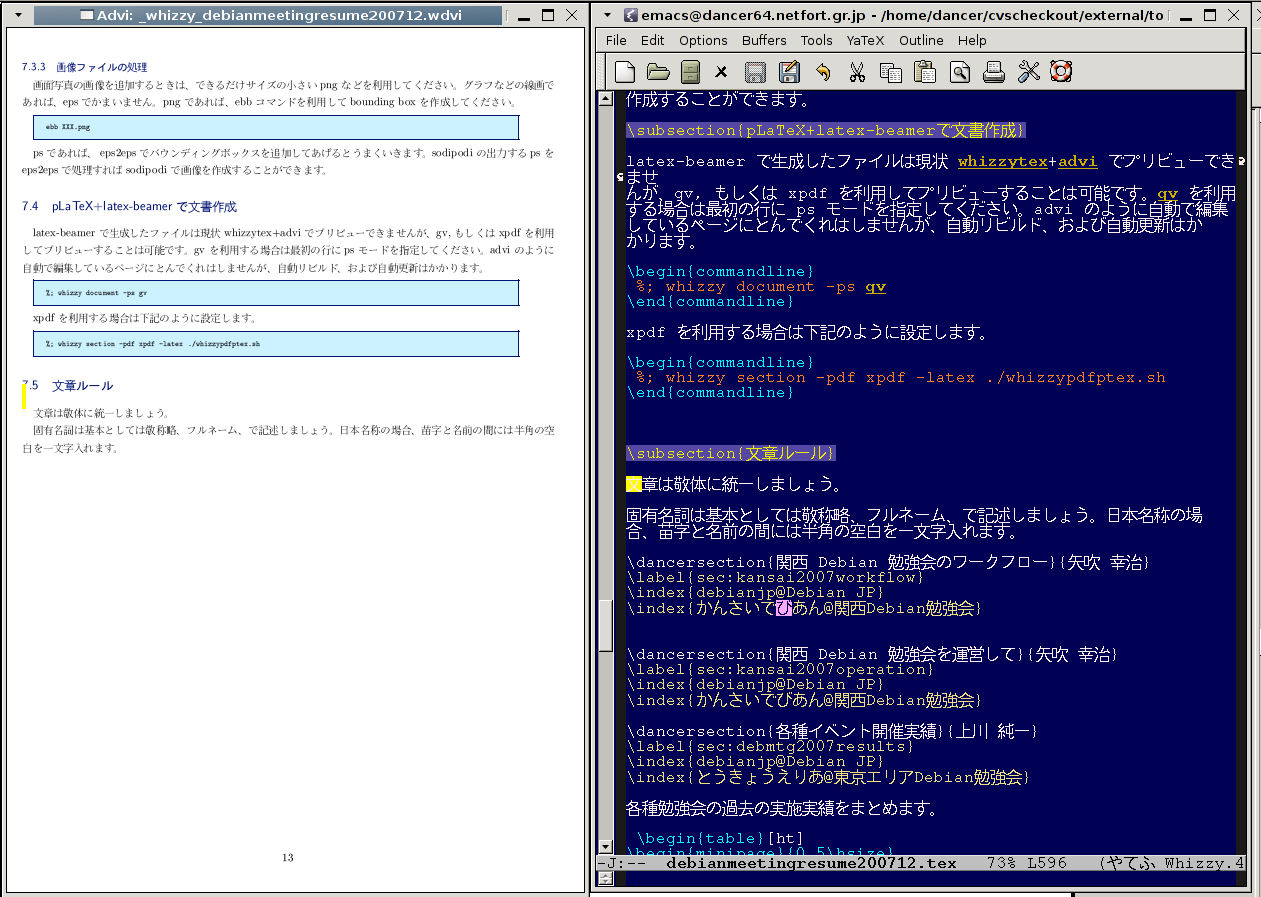
\includegraphics[width=1\hsize]{image200712/whizzytex.png}


\dancersection{関西 Debian 勉強会}{山下 尊也}
\label{sec:kansai2007operation}
\index{debianjp@Debian JP} 
\index{かんさいでびあん@関西Debian勉強会}

\subsection{関西 Debian 勉強会を運営して}

この1年間、いろいろな人の支えがあって勉強会が成立したのだと、12月の忘年
会が終わった後の私の率直な感想です。
9月に矢吹さんから私に担当が変わり、最初は運営の方でかなり悩んでいました。
だって、宴会の幹事とかやった事がない20歳になったばかりの担当者ですから。
しかし、回を重ね、それらは宴会などで運営についての会話を続ける事により、
お互いが理解出来る状態になれたと思います。そのため、来年の目標は、「長続
きできる勉強会」と言うテーマで運営していきます。

一人の力で運営を行うと、その一人が忙しくなった場合などに対応できず、バト
ンパスさえも難しい状況に陥ります。しかし、日頃から分
担して作業を行なっていれば、これからも継続出きるでしょう。

また、Debianについてもっと知りたいと言う事で、関西Debian勉強会の有志で
関西Debian勉強会とは独立した形で、週に一度、読書会(KDR)を開いています。
東京と色は違いますが、関西なりの色で私たち関西Debian勉強会は、より多く
Debianを愛する人で集い、勉強し、お互いが成長出来る勉強会にしたいと考えて
います。

\subsection{関西 Debian 勉強会のワークフロー}

では、感想を述べたところで、実際のワークフローについて紹介します。

関西Debian勉強会では、東京エリアDebian勉強会と同様に、Debian JP の IRC定
例会議に参加し、報告はしていますが、IRC 会議に出れる関西Debian勉強会のメ
ンバーが少ないため、主に幹事用のメーリングリストを利用して進捗の管理をし
ています。まだ、確立出来てない部分もあり、最後の一週間はとてもタイトにな
ります。この一年で関西なりに工夫したワークフローです。東京のワークフロー
を参考に作成しました。関西Debian勉強会では、共有作業の利便性の面でGoogle
ドキュメントで管理しています。

\begin{description}
\item[会場確保] ほとんどの会場は、3ヶ月前から予約の受付が始まります。
	   関西Debian勉強会は土日の午後を予約するため、2ヶ月前にはほとんど
	   の場所が予約で埋まってしまいます。そのため、企画が決定するより前に会場
	   を確保します。会場の料金支払いについては、前日までに入金すれば良いなど比較
	   的融通効くので、とりあえず会場を確保します。また、プロジェ
	   クターを利用する場合は会場確保の段階で伝えておかないと、当日
	   借りる事が出来ない場合もあります。気をつけましょう。
\item[企画立案] 企画を立案します。前回の勉強会の宴会で大抵決定します。12
	   月の忘年会で、どこらへんでお願いするかなどをお願いしておきます。
\item[講師確保] 前回の勉強会の宴会であたりをつけて、講師候補のメールで調
	   整するようにします。
\item[資料作成依頼] 資料の作成を講師に依頼します。
\item[資料作成] 講師が資料を作成します。
\item[資料編集] 資料を集めて資料を編集します。関西Debian勉強会では、講師
	   の負担を軽減するため、\LaTeX{}に限定はしておりません。そのた
	   め、OpenOfficeでの提出も可能です。
\item[印刷向け編集] 利便性の向上のため、PDFで結合します。
	   pdftk\footnote{\url{http://packages.debian.org/sid/pdftk}}などを使
	   うと良いでしょう。
\item[印刷] kinkos\footnote{\url{http://www.kinkos.co.jp/}} やカンプリ
	   \footnote{\url{http://www.kanpuri.co.jp/}}などの業者さんに持って行
	   きます。カンプリの場合は、メンバー割引があり、kinkosの場合は、
	   学生割引があります。開催者側の予定が合わない場合は、kinkosに
	   Webから印刷を依頼する事をを検討しても良いかもしれません。
\item[事前課題設定] 関西Debian勉強会では、基本的に参加者の敷居を下げるために事前課題
	   の設定はしておりません。ただし、希望などがある際は、MLで相談して事前
	   課題を設定します。
\item[事前課題提示] 事前課題をWikiに提示します。
\item[資料反映] 資料に反映します。
\item[案内文文章案作成] 案内文の作成をします。文面は前回の勉強会の時に使っ
	   たものを再利用して加工したものに対してMLで手直しを依頼します。
\item[案内文確定] 手直しなどがなくなったら、案内文を確定します。
\item[mixi掲載] mixiのdebianコミュニティ\footnote{\url{http://mixi.jp/view_community.pl?id=95}}と、
Debian初心者!コミュニティ\footnote{\url{http://mixi.jp/view_community.pl?id=958407}}
に投げます。また、女性のLinux使いコミュニティ\footnote{\url{http://mixi.jp/view_community.pl?id=513105}}に投げてもらうために、女性の方に依頼します。
\item[イベント管理システムの作成] 参加者が参加申し込みのためのフォームを
	   作成します。cotocoto京都\footnote{\url{http://cotocoto.jp}}などを利用し、
	   debian-users,debian-develに投稿する前には作成しておきます。
\item[debian-users,debian-devel投稿] Debian JPのメーリングリスト\footnote{\url{debian-users@debian.or.jp},\url{debian-devel@debian.or.jp},}
に投稿します。二週間前ごろをメドにします。
\item[debian-users,debian-devel再度投稿] 一週間前ごろをメドにします。ここ
で変更すべき内容は変更を行い、当日の予定とします。
\item[DebianJPページ] DebianJP会員が、DebianJPのイベントのページを更新します。
\item[参加者把握] 数日前に参加者を把握しておきます。
\item[出席簿印刷] 当日か前日に出席簿を印刷します。
\item[宴会予約] 宴会の場所を予約します。店に電話で直接連絡します。
最近の参加者の意見として、4000円以内に収まる事が望ましいみたいです。
\item[宴会費回収] 宴会の最後に、代金を回収します。
関西Debian勉強会では、講師の方と学生については1000円引きを実施しています。
\item[会場設置] 事前に幹事がはやめに入ることが必要です。
開始時刻よりも前から会場を取っているので、30分ほど前には集まり、会場を設
置します。
\item[出席確認] 出席を確認します。幹事と講師はプロジェクターの設置などで忙しいため、それ
以外の方にやっていただきます。
\item[結果報告書整理] Debian wiki\footnote{\url{http://www.debian.org}}の
	   関西Debian勉強会のページに反応集があるので、そこに記述を行いま
	   す。まだ Debian Wiki のアカウントを持っていない方は、今後のた
	   めに、アカウントを取っておきましょう。また、結果はDebianJP定例
	   会議や、次の勉強会で発表します。
\item[資料公開] Debian wiki\footnote{\url{http://www.debian.org}}の関西Debian
	   勉強会のページに資料を公開します。
\end{description}

\dancersection{各種イベント開催実績}{上川 純一}
\label{sec:debmtg2007results}
\index{debianjp@Debian JP} 
\index{とうきょうえりあ@東京エリアDebian勉強会}

各種勉強会の過去の実施実績をまとめます。
東京エリアDebian勉強会と、関西Debian勉強会について整理します。
グラフにしてみると\fgref{fig:peoplechart}になります。
\begin{figure}[h]
 \begin{center}
  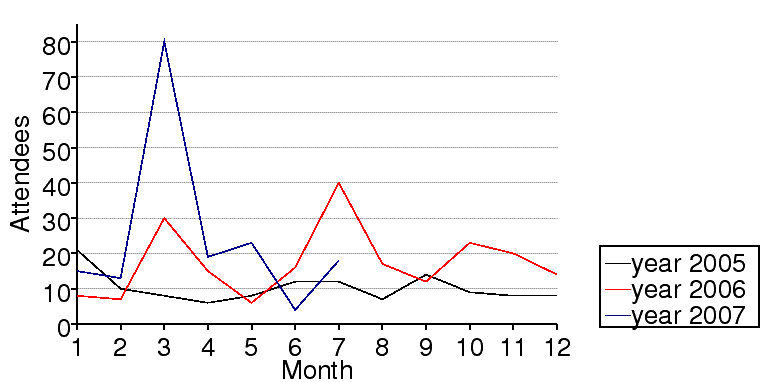
\includegraphics[width=12cm]{image200712/people-chart.png}
 \end{center}
\caption{参加人数推移}
\label{fig:peoplechart}
\end{figure}

表で見てみましょう。
 
 \begin{table}[ht]
\begin{minipage}{0.5\hsize}
 \caption{東京エリアDebian勉強会参加人数(2005年)}\label{tab:count}
 \begin{center}
  \begin{tabular}{|l|c|p{10em}|}
 \hline
   & 人数 & 内容 \\
 \hline
   2005年1月 & 21 & 秘密\\
   2005年2月 & 10 & debhelper1\\
   2005年3月 & 8 &  (早朝) debhelper2、social contract\\
   2005年4月 & 6 & debhelper3\\
   2005年5月 & 8 & DFSG、dpkg-cross、lintian/linda\\
   2005年6月 & 12 & alternatives、d-i\\
   2005年7月 & 12 & toolchain、dpatch\\
   2005年8月 & 7 & Debconf参加報告、ITPからアップロードまで\\
   2005年9月 & 14 & debconf\\
   2005年10月 & 9 & apt-listbugs、バグレポート、debconf翻訳、debbugs\\
   2005年11月 & 8 & DWN翻訳フロー、statoverride\\
   2005年12月 & 8 & 忘年会\\
 \hline
  \end{tabular}
 \end{center}
\end{minipage}
\begin{minipage}{0.5\hsize}
 \caption{東京エリアDebian勉強会参加人数(2006年)}\label{tab:count2006}
 \begin{center}
  \begin{tabular}{|l|c|p{10em}|}
 \hline
 & 参加人数 & 内容\\
 \hline
 2006年1月 & 8 & policy、Debian勉強会でやりたいこと\\
 2006年2月 & 7 & policy、multimedia \\
 2006年3月 & 30 & OSC: debian勉強会、sid \\
 2006年4月 & 15 & policy、latex \\
 2006年5月 & 6 & mexico \\
 2006年6月 & 16 & debconf、cowdancer\\
 2006年7月 & 40 & OSC-Do: MacBook Debian \\
 2006年8月 & 17 & 13執念 \\
 2006年9月 & 12 & 翻訳、Debian-specific、oprofile \\
 2006年10月 & 23 & network、i18n会議、Flash、apt \\
 2006年11月 & 20 & 関西開催: bug、sid、packaging \\
 2006年12月 & 14 & 忘年会 \\
 \hline
  \end{tabular}
 \end{center}
\end{minipage}
 \end{table}

\begin{table}[t]
\begin{minipage}{0.5\hsize}
 \caption{東京エリアDebian勉強会参加人数(2007年)}\label{tab:count2007}
 \begin{center}
  \begin{tabular}{|l|c|p{10em}|}
 \hline
 & 参加人数 & 内容\\
 \hline
2007年1月 & 15 & 一年を企画する \\
2007年2月 & 13 & dbs, dpatch\\ 
2007年3月 & 80 & OSC仮想化 \\
2007年4月 & 19 & quilt, darcs, git\\
2007年5月 & 23 & etch, pbuilder, superh \\   
2007年6月 & 4 & エジンバラ開催:Debconf7 実況中継 \\
2007年7月 & 18 & Debconf7 参加報告\\
2007年8月 & 25 & cdn.debian.or.jp \\   
2007年9月 & 14 & exim \\   
2007年10月 & 30 & OSC Tokyo/Fall(CUPS) \\   
2007年11月 & 19 & live-helper, tomoyo linux kernel patch, server\\
2007年12月 & 11 & 忘年会\\
 \hline
  \end{tabular}
 \end{center}
\end{minipage}
\begin{minipage}{0.5\hsize}
 \caption{関西Debian勉強会参加人数(2007年)}\label{tab:count2007kansai}
 \begin{center}
  \begin{tabular}{|l|c|p{10em}|}
 \hline
 & 参加人数 & 内容 \\
 \hline
2007年3月 & 19 & 開催にあたり \\
2007年4月 & 25 & goodbye、youtube、プロジェクトトラッカー\\
2007年6月 & 23 & 社会契約、テーマ、debian/rules、bugreport\\
2007年7月 & 20前後 & OSC-Kansai \\
2007年8月 & 20 & Inkscape、patch、dpatch\\
2007年9月 & 16 & ライブラリ、翻訳、debtorrent\\
2007年10月 & 22& 日本語入力、SPAMフィルタ\\
2007年11月 & 20前後 & KOF \\   
2007年12月 & 15& 忘年会、iPod touch\\   
 \hline
  \end{tabular}
 \end{center}
\end{minipage}
\end{table}

\clearpage 
\dancersection{東京エリアDebian勉強会の3年間で生まれたDebian
Developerは?}{上川 純一}
\label{sec:debmtg2007-3yearsummary}
\index{とうきょうえりあ@東京エリアDebian勉強会}

Debian 勉強会はなんだかんだといって、3年間実施してきました。Debian勉強会
の当初の目標はばりばりとした開発者の育成をめざすところにあったはずです。
直接的に計測するのは難しいですが、例えばDebian Developer ではなかった人が
開発をする上での支援ができれば目標にそった活動ができていたといえるのでは
ないでしょうか。では、確認してみましょう。

残念ながら Debian 勉強会のおかげで Debian Developer になったと言える人は
まだいないようです。Debian勉強会の参加者で、まだ Debian Developer でない
人たちで、担当パッケージをもっている人たちを任意に抽出してその状況を確認
してみました。

\begin{itemize}
 \item
      山根さん
      \url{http://qa.debian.org/developer.php?login=henrich@debian.or.jp} \\
      eclipse-nls-sdk、jd、ttf-kiloji、ttf-konatu、ttf-vlgothic メンテナ
      ンス中
 \item
      岩松さん
      \url{http://qa.debian.org/developer.php?login=hemamu@t-base.ne.jp}
      \url{http://qa.debian.org/developer.php?login=iwamatsu@nigauri.org} \\
      \footnote{岩松さんがなぜ二つもメールアドレスを使い分けてるのかは不
      明です。}
      linux-uvc、xfonts-mona、libflash、tinywm メンテナンス中
 \item
      小林さん
      \url{http://qa.debian.org/developer.php?login=nori1@dolphin.c.u-tokyo.ac.jp} \\
      orpheus、serf、skkdic、skksearch メンテナンス中
 \item
      三塚さん
      \url{http://qa.debian.org/developer.php?login=mitsuka@misao.gr.jp} \\
      canna メンテナンス中
 \item
      矢吹さん
      \url{http://qa.debian.org/developer.php?login=yabuki@netfort.gr.jp} \\
      canna-shion、td2planet、yc-el メンテナンス中
 \item
      山本さん
      \url{http://qa.debian.org/developer.php?login=yama1066@gmail.com} \\
      file-kanji メンテナンス中
\end{itemize}

ちなみに、この中でDebianとして一番重要\footnote{popconでの投票結果による}な
パッケージは、 libflash で、その次が canna のようです。

\clearpage

% \dancersection{次回}{}

% 未定です。
% 内容は本日決定予定です。

% 参加者募集はまた後程。

%\printindex

\cleartooddpage

\begin{minipage}[b]{0.2\hsize}
 \definecolor{titleback}{gray}{0.9}
 \colorbox{titleback}{\rotatebox{90}{\fontsize{80}{80} {\gt デビアン勉強会} }}
\end{minipage}
\begin{minipage}[b]{0.8\hsize}

\vspace*{15cm}
\hrule
\vspace{2mm}

\includegraphics[width=2cm]{image200502/openlogo-nd.eps}
\noindent \Large \bf Debian 勉強会資料\\ \\
\noindent \normalfont \debmtgyear{}年\debmtgmonth{}月\debmtgdate{}日 \hspace{5mm}  初版第1刷発行\\
\noindent \normalfont 東京エリア Debian 勉強会 (編集・印刷・発行)\\
\hrule
\end{minipage}

\end{document}
